\documentclass[12pt,a4paper,oneside]{article}
\usepackage[T1]{fontenc}
\usepackage[utf8]{inputenc}
\usepackage{lmodern}
\usepackage[margin=25mm,top=27mm,bottom=27mm,headheight=16pt]{geometry}
\usepackage{amsmath,amssymb,mathtools}
\usepackage{array,booktabs,tabularx,longtable,multirow}
\usepackage{enumitem}
\usepackage{graphicx}
\usepackage{float}
\usepackage{caption}
\usepackage{xcolor}
\usepackage{titlesec}
\usepackage{fancyhdr}
\usepackage{hyperref}
\usepackage{url}
\usepackage{setspace}
\definecolor{navy}{HTML}{153654}
\definecolor{midblue}{HTML}{39759A}
\definecolor{softblue}{HTML}{ECF3F8}
\definecolor{ink}{HTML}{263442}
\definecolor{palegray}{HTML}{F3F6F8}
\definecolor{accent}{HTML}{5A8097}
\hypersetup{colorlinks=true,linkcolor=navy,citecolor=midblue,urlcolor=midblue,pdftitle={Dynamic k-Zero Day Safety Metric for Software-Defined Networks: Master's Research Proposal},pdfauthor={Sam Measar Nasser Measar}}
\titleformat{\section}{\Large\bfseries\color{navy}}{\thesection}{0.8em}{}[\vspace{-0.35em}\color{midblue}\titlerule]
\titleformat{\subsection}{\large\bfseries\color{navy}}{\thesubsection}{0.7em}{}
\titleformat{\subsubsection}{\normalsize\bfseries\color{ink}}{\thesubsubsection}{0.65em}{}
\titlespacing*{\section}{0pt}{1.1em}{0.65em}
\titlespacing*{\subsection}{0pt}{0.85em}{0.35em}
\setlength{\parindent}{0pt}
\setlength{\parskip}{0.43em}
\setstretch{1.12}
\emergencystretch=2em
\setlist[itemize]{topsep=3pt,itemsep=2pt,leftmargin=1.6em}
\setlist[enumerate]{topsep=3pt,itemsep=3pt,leftmargin=1.9em}
\captionsetup{font=small,labelfont={bf,color=navy},textfont=it,justification=centering}
\renewcommand{\arraystretch}{1.18}
\pagestyle{fancy}
\fancyhf{}
\fancyhead[L]{\footnotesize\color{ink} Dynamic k-Zero Day Safety for SDN}
\fancyhead[R]{\footnotesize\color{ink} Master's Research Proposal}
\fancyfoot[C]{\footnotesize\thepage}
\renewcommand{\headrulewidth}{0.35pt}
\renewcommand{\footrulewidth}{0pt}
\setcounter{secnumdepth}{3}
\setcounter{tocdepth}{2}
\newcommand{\kw}[1]{\textbf{#1}}
\newcommand{\sourcecaption}[1]{\par\vspace{-0.1em}{\centering\scriptsize\color{accent} #1\par}}
\begin{document}
\hypersetup{pageanchor=false}
\begin{titlepage}
\thispagestyle{empty}
\begin{center}
\vspace*{1.15cm}
{\fontsize{15}{19}\selectfont\color{navy}\bfseries SANA'A UNIVERSITY}\par
\vspace{0.12cm}
{\large\color{ink} Yemen}\par
\vspace{2cm}
{\color{midblue}\rule{0.82\textwidth}{1.35pt}}\par
\vspace{0.5cm}
{\fontsize{22}{27}\selectfont\bfseries\color{navy} Dynamic k-Zero Day Safety Metric\\[0.2cm] for Software-Defined Networks (SDN):\\[0.2cm] Real-Time Risk Assessment and Mitigation}\par
\vspace{0.5cm}
{\color{midblue}\rule{0.82\textwidth}{1.35pt}}\par
\vspace{1.25cm}
{\Large\bfseries Master's Research Proposal}\par
\vspace{0.3cm}
{\normalsize Cyber Security}\par
\vfill
{\normalsize\color{accent} Prepared by}\par
\vspace{0.12cm}
{\Large\bfseries Sam Measar Nasser Measar}\par
\vspace{0.75cm}
{\normalsize Master's Degree in Cyber Security}\par
{\normalsize Sana'a University, Yemen}\par
\vspace{1.15cm}
\end{center}
\end{titlepage}
\hypersetup{pageanchor=true}
\pagenumbering{roman}
\section*{Abstract}
Software-Defined Networking (SDN) offers centralized visibility and programmable forwarding, but frequent topology changes, flow-rule modifications, and controller decisions can invalidate network-risk estimates derived from static configurations. The classical \emph{k-zero day safety} metric estimates a target's resistance to unknown-vulnerability attack chains by counting the minimum number of distinct zero-day vulnerabilities required along a feasible attack path. Its interpretation is attractive for unknown-threat risk reasoning; however, operationalizing the metric under rapidly changing SDN state raises unresolved questions concerning attack-graph maintenance, measurement freshness, uncertainty, and response overhead. This research proposes to design and experimentally assess a \emph{dynamic, SDN-aware} k-zero day safety framework combining controller events and OpenFlow telemetry, incremental attack-graph maintenance, flow-based anomaly evidence, and policy-controlled mitigation. The study will formally specify network-state transitions and a composite risk score, implement a prototype in a Mininet-based laboratory, and compare event-driven incremental assessment against static and full-recomputation baselines. Controlled topology, forwarding-policy, traffic-anomaly, and adversarial-path scenarios will be used to evaluate risk-state consistency, update latency, detection error, operational overhead, and mitigation effectiveness. Because true unknown vulnerabilities cannot be directly enumerated or reliably labeled in a testbed, explicit surrogate assumptions and sensitivity tests will delimit what the findings can establish. The anticipated contribution is a reproducible method for connecting an established structural security metric to timely SDN decisions, together with empirical evidence about its benefits, costs, and limitations. \emph{No implementation or empirical results are claimed in this proposal.}

\noindent\textbf{Keywords:} software-defined networking; k-zero day safety; attack graph; zero-day vulnerability; OpenFlow; anomaly detection; dynamic risk assessment; incremental computation; mitigation; Mininet.

\clearpage
\tableofcontents
\clearpage
\listoffigures
\listoftables
\clearpage
\pagenumbering{arabic}

\section{Introduction and Research Background}\label{sec:intro}
Modern networks are increasingly managed by software that can alter forwarding decisions and security policies with minimal operational delay. SDN separates the application, control, and data planes: applications express management intent, controllers translate policies into device operations, and programmable switches forward traffic according to installed flow rules \cite{mckeown2008openflow,nadeau2013sdn}. This separation offers a coherent vantage point for monitoring and enforcing network security but concentrates critical privileges in the control plane. A successful attack on a controller, a rule-management interface, or a permitted communication path can consequently affect many hosts at once.

A zero-day vulnerability is an unknown weakness whose exploitation cannot be modeled using a complete list of disclosed weaknesses. Conventional vulnerability-counting approaches therefore provide only a partial picture of exposure. Wang and colleagues introduced k-zero day safety to describe the \emph{minimum number of distinct unknown vulnerabilities} that an attacker must exploit to compromise a designated asset \cite{wang2010kzero,wang2014kzero}. The metric is structural: it considers potential multi-step attack paths instead of claiming to enumerate undisclosed flaws. Subsequent work on network diversity and network attack surface underscores that deployment heterogeneity and reachability influence resistance to unknown attacks \cite{zhang2016diversity,zhang2021surface,manadhata2011surface}.

In an SDN deployment, forwarding-table changes, link failures, host additions, and controller policy actions may rapidly change the feasible paths between an untrusted entry point and a protected asset. A measurement computed from yesterday's topology can be exact for the old state yet wrong for the current one. Anomalous flows can also affect a response decision without changing the underlying structural k-value. This proposal therefore treats \emph{structural safety}, \emph{behavioral suspicion}, and \emph{operational mitigation} as related but distinct quantities that must be updated and evaluated together.

\begin{figure}[htbp]
\centering
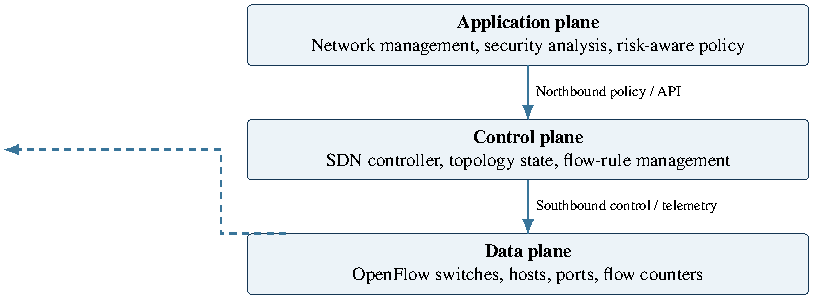
\includegraphics[width=0.97\linewidth,height=8.0cm,keepaspectratio]{figures/diagram_1.pdf}
\caption{The three SDN planes and the information/control interfaces relevant to the proposed study.}
\label{fig:sdnplanes}
\sourcecaption{Author-created conceptual schematic; informed by \cite{mckeown2008openflow,nadeau2013sdn}.}
\end{figure}

\section{Problem Statement}\label{sec:problem}
Classical k-zero day safety assumes that the network state represented by the attack model is sufficiently stable during the assessment. SDN violates that operational premise when flow rules and connectivity change more frequently than the risk model is refreshed. A static assessment may report that a critical target requires several independent unknown exploits while a recently installed flow rule exposes a shorter path. Conversely, a deleted rule might remove a dangerous path, but a stale assessment may continue to report excessive risk. Neither case can be resolved by improving anomaly detection alone, because \emph{topological safety} is not equivalent to \emph{traffic abnormality}.

A viable dynamic approach must overcome four linked technical challenges. First, it must translate controller and data-plane observations into a sufficiently accurate time-indexed attack model. Second, it must update affected paths without rebuilding the entire graph after each routine change. Third, it must combine security information without mistaking probabilistic anomaly evidence for verified exploitation of a zero-day flaw. Fourth, it must issue defensible, reversible mitigation actions while keeping controller load and unintended service disruption within acceptable bounds. The central research problem is therefore \emph{how to maintain a timely and interpretable k-zero day safety assessment for changing SDN states, and whether using it to guide mitigation improves measured security outcomes at a tolerable operational cost}.

\section{Research Gap}\label{sec:gap}
Classical k-zero day safety and its efficient approximations provide established structural reasoning for unknown-vulnerability exposure \cite{wang2010kzero,wang2014kzero,albanese2013efficient}. Attack-graph methods support explicit reasoning about compromise preconditions and paths, yet graph construction and updates create correctness and scalability concerns \cite{zenitani2023attack,lallie2020review}. Separately, SDN monitoring and detection studies demonstrate that flow counters and machine-learning techniques can support anomaly detection, but their performance depends on the selected features, data distribution, and false-positive tolerance \cite{dey2020sdn,sultana2019survey,faezi2023survey}. Controller security work, including AVANT-GUARD, addresses switch-flow and control-plane exposure but does not by itself establish a time-indexed k-zero day safety measurement \cite{shin2013avantguard}.

These lines of research motivate an \emph{integration and validation gap}: there is a need to specify and evaluate a practical method that (i) maintains a target-focused k-value consistently with SDN events, (ii) separates structural attack-path evidence from anomaly-derived risk, and (iii) feeds the resulting estimate into a controlled mitigation loop with measurable delay and overhead. This is a \emph{proposed research gap based on the supplied literature}, not a claim that no previous work has addressed related integration. A formal, up-to-date systematic novelty review will be required before any claim of first implementation or global superiority.

\section{Research Aim and Objectives}\label{sec:objectives}
\textbf{Aim.} To design, implement, and experimentally evaluate a dynamic k-zero day safety framework for SDN that links event-aware attack-path assessment to interpretable real-time risk scoring and operationally safe mitigation.

\textbf{Specific objectives.}
\begin{enumerate}[label=\textbf{O\arabic*.}]
\item Formalize an SDN network-state model, attacker assumptions, target selection, and path-based k-value interpretation, including missing data and mathematical edge cases.
\item Develop a controller-integrated collection pipeline that records topology, flow-rule changes, flow counters, and timestamps with reproducible provenance.
\item Design incremental updates to the attack graph and compare the resulting k-values with independent full-graph recomputation for correctness and update cost.
\item Implement a distinct anomaly-severity estimator and an explicitly normalized, explainable composite risk indicator, with uncertainty and sensitivity analysis.
\item Design a risk-driven mitigation policy with bounded actions, approval gates for disruptive changes, rollback, and feedback reassessment.
\item Evaluate the prototype against static, full-recomputation, and detection-only baselines on controlled Mininet scenarios using paired trials and documented metrics.
\end{enumerate}

\section{Research Questions and Hypotheses}\label{sec:rq}
\begin{description}[style=nextline,leftmargin=1.65em,labelwidth=1.2em,itemsep=4pt]
\item[\textbf{RQ1.}] How accurately can a continuously maintained attack graph and target-specific k-value represent controller-observed SDN state transitions, compared with a full recomputation reference?
\item[\textbf{RQ2.}] Under what topology sizes and flow-rule update rates does incremental maintenance reduce assessment latency and resource cost without unacceptable inconsistency?
\item[\textbf{RQ3.}] Does combining structural k-safety, exposure, anomaly severity, asset criticality, and cautious exploitability estimates improve risk-based decision quality relative to structural-only or anomaly-only baselines?
\item[\textbf{RQ4.}] Can policy-constrained mitigation reduce modeled target exposure and response delay without causing excessive false-positive disruption or controller overhead?
\end{description}

The following \emph{testable directional hypotheses} will be evaluated, rather than presumed true:
\begin{itemize}
\item \textbf{H1:} Under identical update streams, incremental assessment has lower median update latency than repeated full attack-graph reconstruction while matching the reference k-values for the modeled graph.
\item \textbf{H2:} On held-out controlled scenarios, risk-informed decisions offer a better detection/mitigation tradeoff than anomaly-only threshold decisions at comparable false-positive budgets.
\item \textbf{H3:} Compared with no mitigation, bounded risk-driven responses reduce modeled reachability or the composite risk of the affected target without a disproportionate reduction in benign-flow service performance.
\end{itemize}
Each hypothesis specifies comparisons; the actual size, direction, and statistical certainty of effects will be determined only after experiments.

\section{Significance of the Research}\label{sec:significance}
Scientifically, the work can clarify the interpretation of structural unknown-vulnerability metrics under continuously changing reachability and provide a reproducible evaluation protocol for incremental security measurements. For network operations, an event-aware estimate could help distinguish a configuration that is structurally dangerous from a behavioral alert that is suspicious but unconfirmed. For incident response, the proposed framework will explore whether SDN policies can translate those distinctions into proportionate and reversible interventions. The goal is not to assert that a computed risk score measures the real probability of a zero-day compromise; it is to assess the usefulness and limitations of an explicit decision-support proxy.

\section{Literature Review and Related Work}\label{sec:literature}
\subsection{Classical k-Zero Day Safety and Network Diversity}
The original metric treats vulnerability uncertainty as a path-structure problem: an attacker must satisfy conditions along some feasible path, and the weakest path determines target safety \cite{wang2010kzero,wang2014kzero}. Related computational work addresses the cost of estimating this property in larger configurations \cite{albanese2013efficient,wang2017resilience}. Network diversity analyses add the insight that repeated exposure to a common weakness can reduce effective independence among attack steps \cite{zhang2016diversity}; therefore, this proposal will count \emph{distinct assumed vulnerabilities}, not merely hops or edges. Network attack-surface studies additionally motivate measuring exposed routes and services apart from the minimum chain length \cite{zhang2021surface,manadhata2011surface}.

\subsection{Attack Graphs and Lateral Movement}
An attack graph represents attacker preconditions, privilege states, and feasible transitions. The literature describes different graph semantics and algorithms, which makes a precise choice of node and edge interpretation essential \cite{zenitani2023attack,lallie2020review}. Lateral movement provides an operational scenario for testing whether newly reachable intermediate hosts change paths to a high-value target \cite{smiliotopoulos2024lateral}. A fast graph update is not sufficient if it silently omits dependencies created by a new rule; exact comparison against a reference model is therefore a core evaluation requirement.

\subsection{SDN Security and Flow-Based Detection}
OpenFlow provides programmability and switch telemetry but also exposes control-plane stress and policy-enforcement challenges \cite{mckeown2008openflow,shin2013avantguard}. Security monitoring studies show the promise of flow-derived features, including packet and byte counts, duration, and traffic distributions \cite{dey2020sdn,sultana2019survey}. Broad anomaly-detection and cybersecurity-ML reviews warn that rare behavior, class imbalance, and distribution shifts complicate interpretation \cite{chandola2009anomaly,buczak2016survey}. Deep models may detect complex patterns but can create explainability and reproducibility challenges \cite{lecun2015deep,faezi2023survey}. Reviews specific to zero-day detection emphasize that a classifier's success on \emph{held-out attack families} is not equivalent to proving the detection of truly undisclosed vulnerabilities \cite{guo2023zeroday}.

\subsection{Dynamic Risk Measurement and the Remaining Opportunity}
The literature supports attack-path scoring and anomaly monitoring as separate mechanisms, but a prototype that couples SDN event semantics, incremental path correctness, an explicitly bounded score, and rollback-aware mitigation still needs to demonstrate practical utility under a common evaluation protocol. This proposal will use interpretable statistical detectors as baselines; optional clustering and time-series analysis may be tested if the collected data justify them \cite{macqueen1967methods,box2015timeseries,estan2002traffic}. These techniques are \emph{candidates}, not selected or validated findings.

\begin{table}[htbp]
\centering\small
\caption{Positioning of the proposed research against relevant lines of work.}\label{tab:position}
\begin{tabularx}{\textwidth}{@{}p{32mm}X X@{}}
\toprule
\textbf{Research line} & \textbf{Established focus} & \textbf{Question taken forward}\\\midrule
k-zero day safety \cite{wang2014kzero} & Minimum distinct unknown vulnerabilities along an attack path & State changes, path identity and incremental accuracy \\
Attack graphs \cite{zenitani2023attack} & Compromise preconditions and multi-step routes & Local updates with full-recompute checks \\
SDN security \cite{shin2013avantguard} & Programmable forwarding and control-plane protection & Bounded, auditable policy responses \\
Anomaly detection \cite{dey2020sdn} & Behavioral deviations in network telemetry & Fusion with structural metrics and false-positive cost \\
\bottomrule
\end{tabularx}
\end{table}

\section{Proposed Research Methodology}\label{sec:method}
\subsection{Research Design and Phases}
The study will employ design-science prototyping and controlled quantitative experiments. The prototype will be built and assessed in six iterative phases: (1) formal model and assumptions, (2) telemetry and event acquisition, (3) attack-graph construction and differential updates, (4) anomaly and risk estimation, (5) guarded mitigation, and (6) repeated comparative evaluation. Each phase will produce a testable artifact or specification. The primary independent variables will include network size, topology-change rate, flow-table churn, anomaly intensity, the policy scenario, and risk-scoring configuration. Dependent variables will include assessment latency, path correctness, detection behavior, mitigative impact, and controller overhead.

\begin{figure}[htbp]
\centering
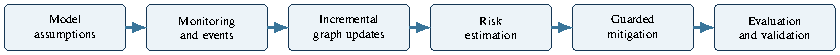
\includegraphics[width=0.97\linewidth,height=8.0cm,keepaspectratio]{figures/diagram_2.pdf}
\caption{Planned research phases, from formal assumptions to comparative evaluation.}\label{fig:phases}
\sourcecaption{Author-created proposed research methodology.}
\end{figure}

\subsection{Experimental Architecture}
A Mininet emulation will host Open vSwitch instances, end hosts, an untrusted ingress segment, application-tier nodes, and one or more critical targets. An open-source controller, initially a Ryu-compatible OpenFlow test environment subject to version and maintenance checks, will maintain the control plane and expose topology and flow-table events. A Python-based research service will collect event records, maintain graph state, run an initial interpretable anomaly model, and compute k-safety and risk. A mitigation adapter will request rule additions, deletions, rate limiting, or segment isolation through controller-approved APIs. A separate experiment orchestrator will generate event sequences and collect ground-truth timestamps. Only laboratory networks under the researcher's control will be used.

\begin{figure}[htbp]
\centering
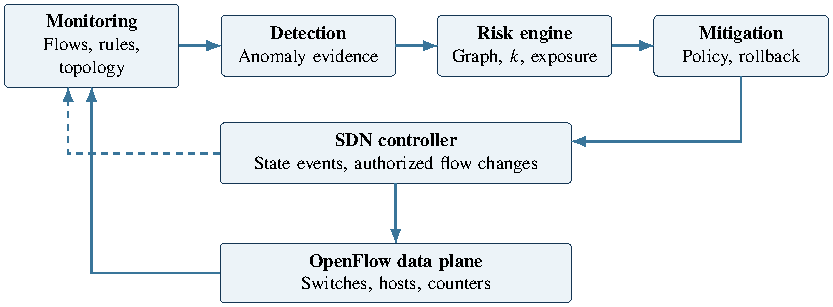
\includegraphics[width=0.97\linewidth,height=8.0cm,keepaspectratio]{figures/diagram_3.pdf}
\caption{Proposed SDN-aware k-zero day safety prototype and closed-loop control architecture.}\label{fig:architecture}
\sourcecaption{Author-created, proposed components; no implementation is claimed.}
\end{figure}

\subsection{Monitoring and Feature Engineering}
The collector will combine switch counters (packet and byte counts, durations, per-port aggregates) with controller-sourced flow-rule modifications, topology observations, and policy logs. It will distinguish a \emph{controller command issued} timestamp from a \emph{switch state observed} timestamp, because command delivery does not guarantee instantaneous installation. Raw cumulative counters will be converted into windowed rates using elapsed time; resets, counter wraparound, duplicate notifications, and missing observations will be detected and flagged. Host- and target-level features will include source/destination diversity, flow churn rate, short-lived connection bursts, and approximate target reachability indicators. Feature extraction will be constrained to metadata that is collectable without inspecting private payloads.

\begin{table}[htbp]
\centering\small
\caption{Proposed telemetry inputs and their interpretation.}\label{tab:features}
\begin{tabularx}{\textwidth}{@{}p{32mm}p{41mm}X@{}}
\toprule
\textbf{Input} & \textbf{Example source} & \textbf{Planned use and limitation}\\\midrule
Flow packets / bytes & OpenFlow statistics & Windowed rates; subject to sampling and counter reset\\
Flow duration / port diversity & Switch and flow metadata & Behavioral context, not proof of malicious traffic\\
Flow adds / deletes & Controller event log & Changes in reachability; requires installed-state confirmation\\
Host/link changes & Controller discovery and link events & Local graph invalidation; delayed discovery may cause stale state\\
Asset importance & Research policy inventory & Criticality weight, preassigned and documented\\
Anomaly severity & Detection engine & Behavioral evidence with calibrated uncertainty\\
\bottomrule
\end{tabularx}
\end{table}

\begin{figure}[htbp]
\centering
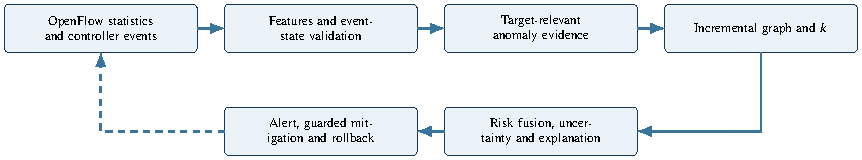
\includegraphics[width=0.97\linewidth,height=8.0cm,keepaspectratio]{figures/diagram_4.pdf}
\caption{Proposed real-time telemetry, feature processing, risk assessment, and feedback workflow.}\label{fig:pipeline}
\sourcecaption{Author-created workflow inspired by the supplied source paper's Figure 6.}
\end{figure}

\subsection{Anomaly Detection and Calibration}
A transparent baseline detector will estimate deviations in normalized flow rates, port diversity, and flow churn relative to benign training windows. Robust z-score or quantile thresholds will provide a simple, explainable benchmark. If the data volume and class separation justify them, a second method (for example, isolation-based outlier detection or clustering) may be trained and compared. Training will use one set of time windows/topologies; threshold selection will use a separated validation set; and final reporting will use held-out scenario seeds and, where feasible, entire unseen traffic families. Label leakage will be prevented by grouping temporally related flows within the same experimental split. Output $A_{\mathrm{sev}}(T,t)\in[0,1]$ will be a calibrated \emph{anomaly severity}, not a confirmed zero-day probability.

\subsection{Dynamic Attack-Graph Representation}
The model will define vertices for attacker-controlled entry conditions, host/service access, privilege states, and protected targets. Edges will represent transitions possible under assumed attack prerequisites and observed connectivity. A topology or flow-rule event will first update a reachability dependency map; this will trigger invalidation and regeneration of impacted exploit-possibility edges. All graph events will be versioned by observation time and sequence number. Every event batch will produce (i) an incremental graph and (ii) an independent periodically recomputed reference graph. A mismatch will be logged with the smallest divergent set of nodes/edges, ensuring that speed cannot substitute for accuracy.

For zero-day assumptions, the prototype will use predeclared \emph{hypothetical exploit opportunities} associated with reachable services or software-diversity classes. They are not asserted to correspond to undisclosed real vulnerabilities. Where multiple steps share the same assumed vulnerability identifier, that identifier will be counted only once. The study will vary these assumptions and show whether its comparative findings are stable under alternative mappings.

\subsection{Incremental Update Strategy}
The initial algorithm will maintain a mapping between network objects (switch ports, rule predicates, hosts, and services) and the attack-graph edges that depend on them. For each new event, it will identify affected dependency objects, invalidate relevant graph edges, apply replacement edges, and update only target-reachable portions of the graph. A target's $k$-value will be invalidated if any of its candidate minimizing paths could change; otherwise the previous value may be reused with an explicit consistency check. A full rebuild will be run on a configurable audit schedule, and always after a detected inconsistency. The implementation will record the number of updated nodes and edges, the time spent in each stage, and the fraction of events that require a full recomputation.

\begin{figure}[htbp]
\centering
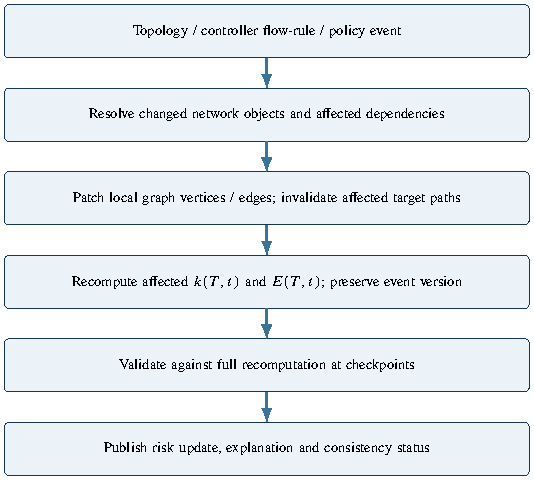
\includegraphics[width=0.97\linewidth,height=8.0cm,keepaspectratio]{figures/diagram_5.pdf}
\caption{Proposed incremental attack-graph update and consistency-check procedure.}\label{fig:graphupdate}
\sourcecaption{Author-created conceptual sequence, adapted in meaning from the supplied paper's Figure 5.}
\end{figure}

\subsection{Risk Estimation and Decision Policy}
The composite score will be calculated only after input timestamps, normalization, and data-confidence tags have been checked. The score will report each contributing term, the current minimum path assumptions, a data-freshness age, and a confidence status. A mitigation policy will map \emph{empirically calibrated} decision regions to candidate actions. Initial thresholds, if needed during development, will be declared provisional and excluded from inferential claims. For critical targets, destructive actions such as segment isolation will require human authorization or a narrowly defined emergency rule. Automated actions will carry expiry timers, rule-priority checks, logging, and rollback instructions. Repeated flapping between actions will be reduced using hysteresis and minimum hold times.

\section{Proposed Mathematical Model}\label{sec:model}
\subsection{Network State and Attack Paths}
Let the time-indexed network state be
\begin{equation}
S(t)=\bigl(V(t),L(t),F(t),Q(t),H(t)\bigr),\label{eq:state}
\end{equation}
where $V(t)$ represents observed devices and hosts, $L(t)$ active links, $F(t)$ effective forwarding rules, $Q(t)$ controller/security policies, and $H(t)$ observed host/service properties. Let $T$ be a protected asset and $\mathcal{A}$ the defined attacker entry conditions. The attack graph $G(S(t),\mathcal{A})$ encodes feasible exploit preconditions under the modeling assumptions. $P(T,t)$ denotes its set of paths from $\mathcal{A}$ to compromise of $T$.

For each path $p$, let $Z(p)$ be the \emph{set of distinct hypothetical unknown-vulnerability identifiers} on that path, and let $z(p)=|Z(p)|$. The source paper's structural k-zero day formulation is preserved:
\begin{equation}
\boxed{k(T,t)=\min_{p\in P(T,t)}z(p).}\label{eq:k}
\end{equation}
A large finite $k$ represents a structural requirement for more distinct unknown exploits; it is \emph{not} a measured probability of compromise. Counting only edges would be incorrect when one hypothetical vulnerability enables more than one step. As a modeling convention, $P(T,t)=\varnothing$ will produce $k(T,t)=\infty$ (unreachable within the defined graph and assumptions), not a claim of absolute security. If a reachable path requires no assumed zero-day flaw, then $k(T,t)=0$ and the target is already exposed by a modeled known-only path.

\subsection{Exposure, Anomaly Severity, Criticality, and Exploitability}
The exposure term $E(T,t)\in[0,1]$ will be a normalized function of attacker-to-target reachability, exposed services, and path multiplicity. Its definition will be fixed before final testing; one candidate is a weighted combination of normalized reachable-entry count, exposed-service fraction, and capped path-diversity indicators. Normalization constants will come from the training environment or predefined design limits, rather than from the test outcome itself. The detection term $A_{\mathrm{sev}}(T,t)\in[0,1]$ will represent anomaly severity relevant to the target; $C(T)\in[0,1]$ will represent preassigned asset criticality; and $X(T,t)\in[0,1]$ will be a documented heuristic for exploit-opportunity evidence or uncertainty. In the absence of verifiable threat intelligence, $X$ will not be described as a true exploitation probability.

\subsection{Original Conceptual Composite Score}
The source document supplies the following \emph{illustrative}, unvalidated risk equation, here reproduced with asset-specific notation only where applicable:
\begin{equation}
R_{\mathrm{src}}(T,t)=w_1\frac{1}{k(T,t)}
+w_2 A_{\mathrm{sev}}(t)+w_3 C(T)+w_4 X(t)+w_5 E(T,t),
\label{eq:sourceRisk}
\end{equation}
subject to $w_i\geq 0$ and $\sum_{i=1}^{5}w_i=1$. In the proposed application, inputs other than $C(T)$ may vary with time. Equation~\eqref{eq:sourceRisk} is \emph{undefined at $k=0$}; it also requires an explicit interpretation for $k=\infty$. Even with nonnegative normalized weights, the expression is not bounded on $[0,1]$ when $k=0$. Therefore it cannot be deployed safely without a defined boundary convention or transformation.

\subsection{Proposed Bounded Refinement and Uncertainty Handling}
This study will evaluate the \emph{proposed mathematical refinement}
\begin{align}
\phi(k)&=\begin{cases}\dfrac{1}{1+k},&k\in\{0,1,2,\ldots\},\\[4pt]0,&k=\infty,\end{cases}\label{eq:phi}\\[3pt]
R_{\mathrm{prop}}(T,t)&=w_1\phi(k(T,t))
+w_2 A_{\mathrm{sev}}(T,t)+w_3 C(T)+w_4 X(T,t)+w_5 E(T,t),
\label{eq:proposedRisk}
\end{align}
where all terms and weights are in $[0,1]$ and the weights sum to one, giving $0\le R_{\mathrm{prop}}\le1$. This transformation is not a validated security law; it is a convenient bounded alternative enabling an explicit interpretation of $k=0$ and graph unreachability. Potential changes to rank-order sensitivity at larger $k$ must be tested. A missing network observation will not be silently treated as zero exposure: the system will instead attach a stale/uncertain status, optionally calculate best- and worst-case bounds, and suppress aggressive automation when confidence is low.

\begin{table}[htbp]
\centering\small
\caption{Mathematical variables, ranges and interpretation.}\label{tab:variables}
\begin{tabularx}{\textwidth}{@{}p{31mm}p{28mm}X@{}}
\toprule
\textbf{Symbol} & \textbf{Domain} & \textbf{Interpretation}\\\midrule
$S(t)$ & Stateful tuple & Controller-observed topology, links, rules, policies and host properties\\
$P(T,t)$ & Path set & Modeled paths from attacker assumptions to target $T$\\
$k(T,t)$ & $\mathbb{N}_0\cup\{\infty\}$ & Fewest distinct assumed zero-day opportunities on any path\\
$E(T,t)$ & $[0,1]$ & Normalized attack-surface exposure proxy\\
$A_{\mathrm{sev}}(T,t)$ & $[0,1]$ & Target-relevant anomaly severity, not confirmed zero-day exploitation\\
$C(T)$ & $[0,1]$ & Preassigned asset criticality\\
$X(T,t)$ & $[0,1]$ & Explicit, uncertain exploit-opportunity heuristic\\
$w_1,\ldots,w_5$ & $\ge0$, sum $1$ & Calibrated or policy-selected weights\\
$R_{\mathrm{prop}}(T,t)$ & $[0,1]$ & Proposed composite decision-support score\\
\bottomrule
\end{tabularx}
\end{table}

\subsection{Path Computation and Computational Tradeoffs}
Unlike ordinary shortest-path problems, minimizing the number of \emph{distinct labels} along a path is not generally equivalent to minimizing the number of weighted edges, because a shared hypothetical flaw may occur multiple times. The prototype will use an exact method for small graphs (bounded search or set-state dynamic programming where tractable), then explore search pruning or approximation with recorded deviation for larger graphs. An approximation will not be reported as the exact classical k-value. The study will distinguish the computational cost of updating graph structure from the cost of recomputing minimum distinct-label paths and assess both independently. This distinction is essential for a defensible scalability claim.

\section{Proposed System Architecture}\label{sec:system}
The proposed system will be organized around five interfaces, with explicit ownership and versioning. The \emph{state interface} receives controller-verified topology and rule events; the \emph{telemetry interface} receives sampled switch counters; the \emph{detection interface} publishes time-stamped severity and evidence; the \emph{assessment interface} publishes graph version, $k(T,t)$, exposure, risk components, freshness and explanation; and the \emph{enforcement interface} submits a bounded, auditable proposed action to the controller. Distinct interfaces will prevent behavioral alarms from being silently translated into assumptions about unknown vulnerabilities.

\begin{figure}[htbp]
\centering
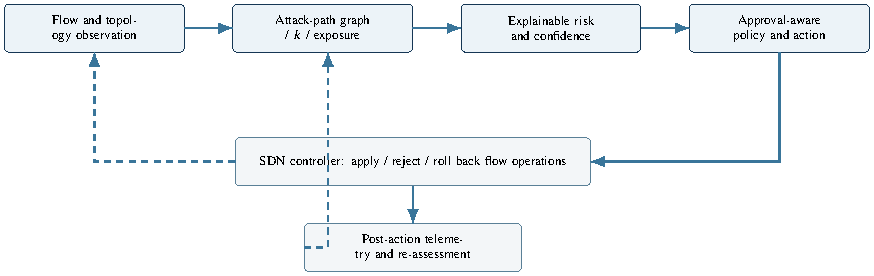
\includegraphics[width=0.97\linewidth,height=8.0cm,keepaspectratio]{figures/diagram_6.pdf}
\caption{Proposed mitigation decision, enforcement, rollback and feedback interfaces.}\label{fig:mitigation}
\sourcecaption{Author-created conceptual diagram of the planned control loop.}
\end{figure}

The framework will operate in three modes: \emph{monitor-only} (calculate and log without altering flow rules), \emph{assisted} (prepare an action for operator approval), and \emph{constrained automatic} (execute only allowlisted, reversible, low-impact responses). All comparative experiments will begin in monitor-only mode, then proceed to assisted/automatic policies within isolated testbeds once correctness and rollback checks pass. Each mitigation event will store the reason, score decomposition, applicable policy, requested change, observed installation result, time to recovery, and whether the modeled target exposure actually improved.

\section{Experimental Design and Evaluation Plan}\label{sec:experiments}
\subsection{Testbed Configuration and Reproducibility}
The testbed will use Mininet with Open vSwitch, a compatible open-source SDN controller, and independently logged traffic and event generators \cite{lantz2010mininet}. Experimental manifests will capture operating-system image, controller/Mininet/OpenFlow versions, network graph generator seed, resource allocations, switch counts, host counts, policy and access-rule templates, detection threshold configuration, and model version. Traffic generators may use iPerf for benign throughput loads, scripted connection bursts for anomalous patterns, and replayable packet or flow traces when permissible. The chosen controller must support reliable enumeration of effective rules and observable change timestamps; otherwise the architecture will be revised and the limitation documented.

A minimal topology will contain an untrusted host, two application intermediaries, multiple SDN switches, and a critical database target. Larger topologies will vary subnet segmentation and service diversity. Multiple independent scenario families will be generated with fixed random seeds and archived descriptions so that individual results can be recreated. Controlled attacks will be limited to the authorized emulated laboratory, and the study will not deliberately deploy unknown exploits.

\subsection{Experimental Scenarios}
The proposal derives the following scenarios from the source paper's conceptual walkthrough, while extending them into repeatable experiments:
\begin{enumerate}[label=\textbf{S\arabic*.}]
\item \textbf{Stable baseline:} Keep topology and rules fixed, establish benign-flow performance, and measure assessment consistency and idle monitoring overhead.
\item \textbf{Flow-rule shortcut:} Add a rule that opens an alternative path to the protected target; verify whether a modeled shortcut reduces the target's distinct-label $k$ and increases reachability exposure.
\item \textbf{Rule withdrawal and isolation:} Remove the shortcut or isolate the implicated host; verify whether the relevant path disappears, whether graph and controller state agree, and what benign traffic is lost.
\item \textbf{Link failure and rerouting:} Disable a link and force alternate forwarding; test cases in which the new path raises, lowers, or leaves $k$ unchanged.
\item \textbf{Anomaly without path change:} Generate a controlled traffic burst or unusual connection-diversity pattern; test whether anomaly severity can change while $k$ remains constant.
\item \textbf{Host addition and lateral path:} Introduce a reachable intermediary, modify service permissions, and examine the appearance or disappearance of multi-hop modeled paths.
\item \textbf{Flow-table churn and scale:} Increase hosts, switches, rules, and event rates to compare incremental updates, full recomputation, controller CPU/memory, and tail latencies.
\item \textbf{False alert and rollback:} Inject benign-but-unusual traffic to exercise suppression, approval, mitigation expiry, and restoration of legitimate connectivity.
\end{enumerate}

\subsection{Comparison Baselines and Ablations}
Four configurations will run against matched scenario seeds and equivalent traffic loads: \textbf{B0} a fixed snapshot k-value refreshed only at a declared audit interval; \textbf{B1} event-triggered full-graph rebuild and exact recomputation; \textbf{B2} anomaly-only detection with matched action budgets; and \textbf{P} the proposed incremental graph, composite risk, and guarded mitigation system. Additional ablations will disable the anomaly component, the structural component, or automatic mitigation to estimate the contribution and cost of each. The full-rebuild model will serve as an \emph{algorithmic reference} for the same modeling assumptions, not as empirical ground truth about actual unknown vulnerabilities.

\begin{table}[htbp]
\centering\small
\caption{Planned controlled comparisons and their principal purpose.}\label{tab:baselines}
\begin{tabularx}{\textwidth}{@{}p{17mm}p{49mm}X@{}}
\toprule
\textbf{ID} & \textbf{Configuration} & \textbf{Principal question}\\\midrule
B0 & Periodic static snapshot, no event updates & How stale does structural assessment become?\\
B1 & Full rebuild after each event & Can incremental results match an exact reference faster?\\
B2 & Anomaly-only alert/response & Does structural context improve decisions at fixed false-positive cost?\\
P & Incremental graph + risk + guarded mitigation & What is the end-to-end benefit and operational cost?\\
Ablations & Remove one risk term or mitigation stage & Which components materially affect observed outcomes?\\
\bottomrule
\end{tabularx}
\end{table}

\subsection{Experimental Procedure and Statistical Analysis}
Each scenario will begin with a clean, recorded switch/controller state. The orchestrator will synchronize available clocks, warm up traffic, establish a benign reference interval, inject a scripted event at a logged timestamp, and record every relevant stage until assessment and optional mitigation settle. Runs will be paired by topology and traffic seed. A pilot study will estimate event-latency variance and determine a defensible final sample size; the initial plan is at least 20 independent seeds per key scenario, adjusted by pilot-based uncertainty requirements rather than presented as an achieved sample. Medians, interquartile ranges, 95\% confidence intervals (using appropriate bootstrap procedures), and paired differences will be reported. Confidence intervals will be favored over unsupported threshold-based significance claims. Multiple-comparison effects and temporal correlation between nearby flow observations will be addressed in the analysis.

\subsection{Validation of the Mathematical Assumptions}
The path model will be tested with deliberately constructed small graphs for which the exact minimum distinct-label count can be checked manually. The evaluation will vary assumed exploit-opportunity assignment, service diversity, attacker starting position, and missing telemetry to characterize sensitivity. Risk-score weights will be declared before final validation and may be selected via a training/validation split and a predeclared criterion such as decision utility subject to a false-positive budget. A single aggregate score cannot be assumed to be universally calibrated across organizations or topologies. Monotonicity, boundedness, and the effect of high asset criticality when a graph is unreachable will be inspected explicitly.

\section{Performance Evaluation Metrics}\label{sec:metrics}
\subsection{Structural and Temporal Correctness}
\textbf{Graph agreement} will compare the incremental graph with a canonical full rebuild, using edge/vertex differences and target reachability agreement. \textbf{k-agreement} will measure the fraction of event checkpoints with exact equality to the full-recompute reference. \textbf{Assessment update delay} will be the elapsed time between effective state-change observation and publication of a new graph-versioned result. \textbf{Staleness} will be the duration for which a published k-value refers to a superseded verified state. Raw event-time and processing-time distributions will be retained to identify backlogs and out-of-order events.

\subsection{Detection and Mitigation Performance}
For controlled, labeled anomaly episodes (\emph{not genuine zero-day discoveries}), standard classification measures will be calculated:
\begin{equation}
\mathrm{TPR}=\frac{TP}{TP+FN},\qquad
\mathrm{FPR}=\frac{FP}{FP+TN},\qquad
\mathrm{Precision}=\frac{TP}{TP+FP}.\label{eq:detection}
\end{equation}
\textbf{Detection delay} is the first qualifying alert minus the labeled anomaly onset; \textbf{action delay} is the time from eligible risk decision to confirmed switch action; and \textbf{end-to-end response time} is from event onset to confirmed mitigation. For each response, the study will record $\Delta k=k_{\mathrm{post}}-k_{\mathrm{pre}}$ when finite, change in $E(T,t)$, change in $R_{\mathrm{prop}}(T,t)$, number of benign flows disrupted, rollback time, and restoration success. Unreachable-to-reachable transitions will be reported categorically rather than forcing infinity into an arithmetic mean.

\subsection{Operational Overhead and Scaling}
Monitoring cost will include controller CPU, memory, event-handling rate, statistics-request volume, and impact on flow setup time. Data-plane overhead will include throughput change and packet delay under identical offered loads. Attack-graph overhead will include graph size, local update time, exact k computation time, memory use, and the fraction of events triggering a full rebuild. The study will record p50, p95, and p99 end-to-end latency where the number of observations permits stable estimates. Resource consumption will be measured on the same allocated hardware and under identical traffic conditions.

\begin{table}[htbp]
\centering\small
\caption{Metrics, measurements and interpretation safeguards.}\label{tab:evaluation}
\begin{tabularx}{\textwidth}{@{}p{34mm}p{48mm}X@{}}
\toprule
\textbf{Metric} & \textbf{Measurement} & \textbf{Interpretive caution}\\\midrule
Exact k agreement & Matching targets / evaluated checkpoints & Relative to the same assumed graph model only\\
Graph update latency & Observed event to versioned output & Must include queuing and timestamp uncertainty\\
Detection rate / FPR & Labeled anomalous / benign trials & Controlled anomalies are not validated zero-days\\
Mitigation response time & Event onset to installed change & Controller acknowledgment is not always switch confirmation\\
Latency and throughput & Difference from matched benign baseline & Separate policy disruption from measurement overhead\\
Controller CPU / memory & Traced utilization and peak values & Report testbed specifications and concurrent loads\\
Risk and exposure change & Before / after under versioned state & A lower score is not proof of eliminated compromise risk\\
\bottomrule
\end{tabularx}
\end{table}

\section{Expected Results and Anticipated Contributions}\label{sec:contrib}
The study is expected to produce a documented prototype, a formal interpretation of time-indexed k-safety, an incremental graph-update procedure with differential tests, an auditable risk calculation, and an experimental dataset of controller events and controlled traffic scenarios. It may demonstrate reduced update latency relative to full rebuilds in some regimes, but that expectation remains a hypothesis; at high churn, path diversity, or graph complexity, incremental maintenance may perform no better or may incur consistency costs. Similarly, composite scoring may improve the utility of response decisions only if its components are appropriately normalized and the false-positive budget is controlled.

The anticipated scientific deliverables are: \emph{(i)} a precise operational model and edge-case treatment for dynamic structural safety, \emph{(ii)} a reproducible correctness/latency benchmark for event-driven graph updates, \emph{(iii)} an evaluation of whether structural and behavioral evidence complement each other in policy decisions, and \emph{(iv)} documented failure modes, limitations, and guidance on safe deployment boundaries. Findings will be presented as measured tradeoffs rather than as proof that zero-day attacks can be identified with certainty.

\section{Research Limitations and Threats to Validity}\label{sec:limitations}
\textbf{Construct validity.} The count of hypothetical unknown-vulnerability identifiers is a model-dependent proxy; it does not establish how many undisclosed exploitable flaws actually exist. Different mappings of services to exploit opportunities may change rank order, and the test results must expose that sensitivity. The proposed score is a decision-support index, not a calibrated compromise probability unless separately validated against meaningful outcomes.

\textbf{Internal validity.} Controller event ordering, delayed topology discovery, counter resets, traffic generation artefacts, and shared compute resources can bias latency or detection measures. Clean resets, controller-versus-switch timestamp separation, matched baselines, and instrumentation logs will reduce but not eliminate these effects.

\textbf{External validity.} Mininet is a controlled emulator and cannot reproduce all controller deployments, switch ASIC behavior, traffic mixtures, enterprise policies, or multi-controller failures. Positive findings will not be generalized to production without independent validation. A single open-source controller and a single resource configuration could narrow applicability.

\textbf{Statistical validity.} Paired trials may exhibit serial correlation and topology-dependent variability. Pilot-guided replication, seed separation, confidence intervals, and disclosed unsuccessful runs will be necessary. A seemingly large count of individual flows cannot replace independent scenario replicates.

\textbf{Operational risks.} False alarms could lead to unnecessary network blocking. A policy might appear to raise $k$ while causing service denial, or while exposing another target via rerouting. Thus, the evaluator must track multiple assets, service-level impacts, rollback, and stale assessment states as well as the selected target's score.

\section{Research Ethics and Security Considerations}\label{sec:ethics}
All experiments will take place in a dedicated, isolated, researcher-authorized network emulation environment. Simulated attacker starting conditions, traffic bursts, scanning-like behavior, and rule modifications will be confined to the laboratory; the study will not use live production targets, real unauthorized credentials, or exploitation of genuinely unknown vulnerabilities. Packet contents and personal identifiers will not be necessary for the core metrics, and telemetry retained for publication will be minimized and sanitized. Experiment scripts, logs, and controller credentials will be protected using role-limited access. Mitigation functionality will require dry-run testing, allowlists, expiry/rollback capability, and explicit human approval for actions that could disrupt critical services. The researcher will document the exact threat model, assumptions, and any residual safety risks before experiments.

\section{Research Work Plan and Timeline}\label{sec:timeline}
A provisional eight-month plan is proposed, subject to departmental approval, access to hardware, and the results of preliminary trials. The schedule is a planning estimate rather than a declared institutional deadline.

\begin{table}[htbp]
\centering\scriptsize
\caption{Proposed eight-month research schedule (\textbullet{} = active period).}\label{tab:timeline}
\begin{tabularx}{\textwidth}{@{}X*{8}{>{\centering\arraybackslash}p{8mm}}@{}}
\toprule
\textbf{Workstream} & \textbf{M1}&\textbf{M2}&\textbf{M3}&\textbf{M4}&\textbf{M5}&\textbf{M6}&\textbf{M7}&\textbf{M8}\\\midrule
Detailed literature review / protocol & \textbullet&\textbullet&&&&&&\\
Threat model, mathematics, design & \textbullet&\textbullet&\textbullet&&&&&\\
Mininet and telemetry pipeline &&\textbullet&\textbullet&\textbullet&&&&\\
Graph maintenance / exactness tests &&&\textbullet&\textbullet&\textbullet&&&\\
Anomaly/risk model and calibration &&&&\textbullet&\textbullet&\textbullet&&\\
Mitigation safeguards / integration &&&&&\textbullet&\textbullet&&\\
Experiments and statistical analysis &&&&&&\textbullet&\textbullet&\\
Proposal-to-thesis reporting / revision &&&&&&&\textbullet&\textbullet\\
\bottomrule
\end{tabularx}
\end{table}

\subsection{Milestones and Decision Gates}
At the end of Month 2, the formal threat model, exactness-test cases, and implementation plan will be reviewed. At the end of Month 4, the telemetry pipeline and a reference full-rebuild attack model must produce reproducible outputs; otherwise the incremental subsystem will not be declared ready for evaluation. At the end of Month 6, safe mitigation and rollback tests must pass before automatic actions are activated. The final phase will prioritize a reproducible experiment archive and analysis, even if the eventual evidence rejects one or more proposed hypotheses.

\section{Conclusion}\label{sec:conclusion}
This proposal advances a specific, testable investigation of how classical k-zero day safety can be maintained and used in an SDN environment where reachability, policy, and traffic observations change continuously. It preserves the structural meaning of the original metric while introducing an explicitly provisional risk-scoring refinement, a versioned incremental attack-graph design, and a feedback-controlled mitigation architecture. The research will compare proposed and baseline methods using controlled Mininet experiments and will evaluate not only update speed and anomaly recognition but also exactness, operational cost, and unintended disruption. Its contribution will depend on the results of these future experiments. No implementation, validated performance improvement, or real zero-day exploitation detection is claimed at this stage.

\clearpage
\addcontentsline{toc}{section}{References}
% Fast bibliography without Biber/BibTeX; bibliography derived from references.bib.
% Update references here if editing bibliographic details.
\begingroup
\small
\begin{thebibliography}{99}
\bibitem{mckeown2008openflow} Nick McKeown, Tom Anderson, Hari Balakrishnan, Guru Parulkar, Larry Peterson, Jennifer Rexford, Scott Shenker, Jonathan Turner. ``{OpenFlow}: Enabling Innovation in Campus Networks,'' \emph{ACM SIGCOMM Computer Communication Review}, vol.~38, no.~2, pp.~69--74, 2008.

\bibitem{nadeau2013sdn} Thomas D. Nadeau, Ken Gray. \emph{{SDN}: Software Defined Networks: An Introduction}. O'Reilly Media, Sebastopol, CA, 2013.

\bibitem{wang2010kzero} Lingyu Wang, Sushil Jajodia, Anoop Singhal, Steven Noel. ``{k-Zero Day Safety}: Measuring the Security Risk of Networks against Unknown Attacks,'' in \emph{Proceedings of the 15th European Symposium on Research in Computer Security (ESORICS)}, series Lecture Notes in Computer Science, vol.~6345, Springer, pp.~573--587, 2010.

\bibitem{wang2014kzero} Lingyu Wang, Sushil Jajodia, Anoop Singhal, Pengsu Cheng, Steven Noel. ``{k-Zero Day Safety}: A Network Security Metric for Measuring the Risk of Unknown Vulnerabilities,'' \emph{IEEE Transactions on Dependable and Secure Computing}, vol.~11, no.~1, pp.~30--44, 2014.

\bibitem{zhang2016diversity} Ming Zhang, Lingyu Wang, Sushil Jajodia, Anoop Singhal, Massimiliano Albanese. ``Network Diversity: A Security Metric for Evaluating the Resilience of Networks against Zero-Day Attacks,'' \emph{IEEE Transactions on Information Forensics and Security}, vol.~11, no.~5, pp.~1071--1086, 2016.

\bibitem{zhang2021surface} Ming Zhang, Lingyu Wang, Sushil Jajodia, Anoop Singhal. ``Network Attack Surface: Lifting the Concept of Attack Surface to the Network Level for Evaluating Networks' Resilience Against Zero-Day Attacks,'' \emph{IEEE Transactions on Dependable and Secure Computing}, vol.~18, no.~1, pp.~310--324, 2021.

\bibitem{manadhata2011surface} Pratyusa K. Manadhata, Jeannette M. Wing. ``An Attack Surface Metric,'' \emph{IEEE Transactions on Software Engineering}, vol.~37, no.~3, pp.~371--386, 2011.

\bibitem{albanese2013efficient} Massimiliano Albanese, Sushil Jajodia, Anoop Singhal, Lingyu Wang. ``An Efficient Approach to Assessing the Risk of Zero-Day Vulnerabilities,'' in \emph{Proceedings of the International Conference on Security and Cryptography (SECRYPT)}, 2013.

\bibitem{zenitani2023attack} Kengo Zenitani. ``Attack Graph Analysis: An Explanatory Guide,'' \emph{Computers \& Security}, vol.~126, pp.~103081, 2023. doi: \url{https://doi.org/10.1016/j.cose.2022.103081}.

\bibitem{lallie2020review} Harjinder S. Lallie, Kurt Debattista, Jay Bal. ``A Review of Attack Graph and Attack Tree Visual Syntax in Cyber Security,'' \emph{Computer Science Review}, vol.~35, pp.~100219, 2020.

\bibitem{dey2020sdn} S. K. Dey, M. M. Rahman. ``Effects of Machine Learning Approach in Flow-Based Anomaly Detection on Software-Defined Networking,'' \emph{Symmetry}, vol.~12, no.~1, pp.~7, 2020.

\bibitem{sultana2019survey} N. Sultana, N. Chilamkurti, W. Peng, R. Alhadad. ``Survey on {SDN} Based Network Intrusion Detection System Using Machine Learning Approaches,'' \emph{Peer-to-Peer Networking and Applications}, vol.~12, pp.~493--501, 2019.

\bibitem{faezi2023survey} S. Faezi, A. Shirmarz. ``A Comprehensive Survey on Machine Learning Using in Software Defined Networks ({SDN}),'' \emph{Human-Centric Intelligent Systems}, vol.~3, pp.~312--343, 2023.

\bibitem{shin2013avantguard} Seungwon Shin, Vinod Yegneswaran, Phillip Porras, Guofei Gu. ``{AVANT-GUARD}: Scalable and Vigilant Switch Flow Management in Software-Defined Networks,'' in \emph{Proceedings of the ACM SIGSAC Conference on Computer and Communications Security (CCS)}, pp.~413--424, 2013. doi: \url{https://doi.org/10.1145/2508859.2516684}.

\bibitem{wang2017resilience} Lingyu Wang, Sushil Jajodia, Anoop Singhal, Pengsu Cheng, Steven Noel. ``{k-Zero Day Safety}: Evaluating the Resilience of Networks Against Unknown Attacks,'' in \emph{Network Security Metrics}, Springer, Cham, pp.~73--94, 2017.

\bibitem{smiliotopoulos2024lateral} Christos Smiliotopoulos, Georgios Kambourakis, Constantinos Kolias. ``Detecting Lateral Movement: A Systematic Survey,'' \emph{Heliyon}, vol.~10, no.~4, pp.~e26317, 2024.

\bibitem{chandola2009anomaly} Varun Chandola, Arindam Banerjee, Vipin Kumar. ``Anomaly Detection: A Survey,'' \emph{ACM Computing Surveys}, vol.~41, no.~3, pp.~1--58, 2009.

\bibitem{buczak2016survey} Anna L. Buczak, Erhan Guven. ``A Survey of Data Mining and Machine Learning Methods for Cyber Security Intrusion Detection,'' \emph{IEEE Communications Surveys \& Tutorials}, vol.~18, no.~2, pp.~1153--1176, 2016.

\bibitem{lecun2015deep} Yann LeCun, Yoshua Bengio, Geoffrey Hinton. ``Deep Learning,'' \emph{Nature}, vol.~521, no.~7553, pp.~436--444, 2015.

\bibitem{guo2023zeroday} Yang Guo. ``A Review of Machine Learning-Based Zero-Day Attack Detection: Challenges and Future Directions,'' \emph{Computer Communications}, vol.~198, pp.~175--185, 2023. doi: \url{https://doi.org/10.1016/j.comcom.2022.11.001}.

\bibitem{macqueen1967methods} J. MacQueen. ``Some Methods for Classification and Analysis of Multivariate Observations,'' in \emph{Proceedings of the 5th Berkeley Symposium on Mathematical Statistics and Probability}, vol.~1, pp.~281--297, 1967.

\bibitem{box2015timeseries} George E. P. Box, Gwilym M. Jenkins, Gregory C. Reinsel, Greta M. Ljung. \emph{Time Series Analysis: Forecasting and Control}. ed.~5, John Wiley \& Sons, Hoboken, NJ, 2015.

\bibitem{estan2002traffic} Cristian Estan, George Varghese. ``New Directions in Traffic Measurement and Accounting,'' \emph{ACM SIGCOMM Computer Communication Review}, vol.~32, no.~4, pp.~323--336, 2002.

\bibitem{lantz2010mininet} Bob Lantz, Brandon Heller, Nick McKeown. ``A Network in a Laptop: Rapid Prototyping for Software-Defined Networks,'' in \emph{Proceedings of the 9th ACM SIGCOMM Workshop on Hot Topics in Networks (HotNets)}, 2010.

\end{thebibliography}
\endgroup

\end{document}
